\documentclass[8pt,aspectratio=169]{beamer}
\usetheme{Madrid}
\usepackage{graphicx}
\usepackage{booktabs}
\usepackage{adjustbox}
\usepackage{multicol}
\usepackage{amsmath}
\usepackage{amssymb}  % For checkmark symbol
\usepackage{tikz}     % For progress indicators

% Color definitions
\definecolor{mlblue}{RGB}{0,102,204}
\definecolor{mlpurple}{RGB}{51,51,178}
\definecolor{mllavender}{RGB}{173,173,224}
\definecolor{mllavender2}{RGB}{193,193,232}
\definecolor{mllavender3}{RGB}{204,204,235}
\definecolor{mllavender4}{RGB}{214,214,239}
\definecolor{mlorange}{RGB}{255, 127, 14}
\definecolor{mlgreen}{RGB}{44, 160, 44}
\definecolor{mlred}{RGB}{214, 39, 40}
\definecolor{mlgray}{RGB}{127, 127, 127}

% Additional colors for template compatibility
\definecolor{lightgray}{RGB}{240, 240, 240}
\definecolor{midgray}{RGB}{180, 180, 180}

% Apply custom colors to Madrid theme
\setbeamercolor{palette primary}{bg=mllavender3,fg=mlpurple}
\setbeamercolor{palette secondary}{bg=mllavender2,fg=mlpurple}
\setbeamercolor{palette tertiary}{bg=mllavender,fg=white}
\setbeamercolor{palette quaternary}{bg=mlpurple,fg=white}

\setbeamercolor{structure}{fg=mlpurple}
\setbeamercolor{section in toc}{fg=mlpurple}
\setbeamercolor{subsection in toc}{fg=mlblue}
\setbeamercolor{title}{fg=mlpurple}
\setbeamercolor{frametitle}{fg=mlpurple,bg=mllavender3}
\setbeamercolor{block title}{bg=mllavender2,fg=mlpurple}
\setbeamercolor{block body}{bg=mllavender4,fg=black}

% Remove navigation symbols
\setbeamertemplate{navigation symbols}{}

% Clean itemize/enumerate
\setbeamertemplate{itemize items}[circle]
\setbeamertemplate{enumerate items}[default]

% Reduce margins for more content space
\setbeamersize{text margin left=5mm,text margin right=5mm}

% Command for bottom annotation (Madrid-style)
\newcommand{\bottomnote}[1]{%
\vfill
\vspace{-2mm}
\textcolor{mllavender2}{\rule{\textwidth}{0.4pt}}
\vspace{1mm}
\footnotesize
\textbf{#1}
}

% Progress indicator command
\newcommand{\progressbar}[1]{%
\begin{tikzpicture}[overlay, remember picture]
\node[anchor=north east, xshift=-5mm, yshift=-5mm] at (current page.north east) {
  \tiny
  \ifcase#1
    \relax % 0: Problem framing
    \textcolor{mlorange}{$\bullet$} \textcolor{mlgray}{$\circ$} \textcolor{mlgray}{$\circ$} \textcolor{mlgray}{$\circ$} \textcolor{mlgray}{$\circ$}
  \or % 1: Lecture 1
    \textcolor{mlgreen}{$\bullet$} \textcolor{mlorange}{$\bullet$} \textcolor{mlgray}{$\circ$} \textcolor{mlgray}{$\circ$} \textcolor{mlgray}{$\circ$}
  \or % 2: Lecture 2
    \textcolor{mlgreen}{$\bullet$} \textcolor{mlgreen}{$\bullet$} \textcolor{mlorange}{$\bullet$} \textcolor{mlgray}{$\circ$} \textcolor{mlgray}{$\circ$}
  \or % 3: Lecture 3
    \textcolor{mlgreen}{$\bullet$} \textcolor{mlgreen}{$\bullet$} \textcolor{mlgreen}{$\bullet$} \textcolor{mlorange}{$\bullet$} \textcolor{mlgray}{$\circ$}
  \or % 4: Lecture 4
    \textcolor{mlgreen}{$\bullet$} \textcolor{mlgreen}{$\bullet$} \textcolor{mlgreen}{$\bullet$} \textcolor{mlgreen}{$\bullet$} \textcolor{mlorange}{$\bullet$}
  \fi
};
\end{tikzpicture}%
}

\title{Week 1: Green Finance Foundations}
\subtitle{Problem-Driven Learning: Climate $\rightarrow$ Markets $\rightarrow$ Valuation $\rightarrow$ Applications}
\author{Green Finance Course}
\date{v3.0 - 4-Lecture Structure with Living Learning Goals}

\begin{document}

% ============================================================
% PROBLEM FRAMING SECTION (Slides 0-2)
% ============================================================

% Slide 0: Climate Crisis
\begin{frame}[t]{The Climate Challenge: Paris Agreement and 2 Degree C Target}
\progressbar{0}
\begin{columns}[T]
\column{0.48\textwidth}
\textbf{Global Climate Commitments}
\begin{itemize}
\item Paris Agreement (2015): Limit warming to 1.5-2 degree C
\item Net-zero targets: 140+ countries by 2050
\item Carbon budget: ~400 GtCO2 remaining for 1.5 degree C
\item Current trajectory: 2.7 degree C warming by 2100
\item Urgent action required: Emissions must halve by 2030
\end{itemize}

\column{0.48\textwidth}
\textbf{Finance Implications}
\begin{itemize}
\item Energy transition investment need: \$4-5 trillion annually
\item Current green investment: ~\$2 trillion annually
\item Annual funding gap: \$2+ trillion
\item Private capital essential to close gap
\item Traditional development finance insufficient
\end{itemize}
\end{columns}
\bottomnote{[Problem] Climate crisis creates urgent need for scaled financial solutions}
\end{frame}

% Slide 1: Funding Gap
\begin{frame}[t]{The Green Finance Investment Gap: Data Puzzle}
\progressbar{0}
\vspace{-10mm}
\begin{center}
\includegraphics[width=0.85\textwidth]{charts/week1/11_investment_gap/11_investment_gap.pdf}
\end{center}
\vspace{-5mm}
\bottomnote{[Problem] Research question: How can capital markets mobilize \$2.04T annual gap?}
\end{frame}

% Slide 2: Green Finance Solution
\begin{frame}[t]{Green Finance: Linking Capital Markets to Climate Action}
\progressbar{0}
\begin{columns}[T]
\column{0.48\textwidth}
\textbf{Market-Based Solution}
\begin{itemize}
\item Channel private capital to environmental projects
\item Use existing financial infrastructure (bond markets)
\item Create specialized instruments (green bonds)
\item Leverage investor ESG preferences
\item Scale beyond public sector capacity
\end{itemize}

\column{0.48\textwidth}
\textbf{This Week's 4-Lecture Journey}
\begin{itemize}
\item Lecture 1: WHY do green finance markets exist? (Theory)
\item Lecture 2: HOW MUCH capital is mobilized? (Measurement)
\item Lecture 3: HOW TO PRICE green instruments? (Valuation Part 1)
\item Lecture 4: WHERE to apply and integrate? (Valuation Part 2 + Applications)
\end{itemize}
\end{columns}
\bottomnote{[Problem] Practical challenge: Design financial mechanisms that are profitable AND impactful}
\end{frame}

% ============================================================
% LECTURE 1: GOAL 1 THEORY (Slides 3-13)
% ============================================================

% Slide 3: Learning Goal 1 Title
\begin{frame}[plain]
\progressbar{1}
\vfill
\centering
\begin{beamercolorbox}[sep=12pt,center]{title}
{\Huge \textbf{Learning Goal 1}}\\[1.5em]
{\Large Understand the market microstructure theory explaining why green finance markets exist and how they function}\\[1em]
{\normalsize \textcolor{mllavender}{theoretical | Foundation - Establishes theoretical basis}}
\end{beamercolorbox}
\vfill
\end{frame}

% Slide 4: Framework Overview
\begin{frame}[t]{Market Microstructure Framework for Green Finance}
\progressbar{1}
\begin{center}
{\large \textbf{Information Asymmetry and Signaling Theory}}
\end{center}
\vspace{0.5em}
\begin{columns}[T]
\column{0.48\textwidth}
\textbf{Core Theoretical Principles}
\begin{itemize}
\item Information asymmetry: Issuers know true environmental impact, investors cannot observe directly
\item Verification as credible signaling mechanism reducing asymmetry
\item Market segmentation by investor ESG preferences
\item Adverse selection risk without credible signals
\end{itemize}
\column{0.48\textwidth}
\textbf{Market Equilibrium Predictions}
\begin{itemize}
\item Greenium emerges from excess demand in segmented market
\item Verification costs create quality differentiation
\item Liquidity premium for standardized green instruments
\item Reputation effects for repeat issuers
\end{itemize}
\end{columns}
\bottomnote{[Goal 1] Theory predicts observable phenomena - We will test these in Lecture 2}
\end{frame}

% Slide 5: Chart - Ecosystem
\begin{frame}[t]{Green Finance Ecosystem: Theoretical Perspective}
\progressbar{1}
\vspace{-13mm}
\begin{center}
\includegraphics[width=0.4\textwidth]{charts/week1/week1_v2_goal1_chart1_ecosystem.pdf}
\end{center}
\vspace{-5mm}
\bottomnote{[Goal 1] Ecosystem structure reflects information asymmetry and signaling needs}
\end{frame}

% Slide 6: Information Asymmetry Problem
\begin{frame}[t]{The Information Asymmetry Problem}
\progressbar{1}
\begin{columns}[T]
\column{0.48\textwidth}
\textbf{Why Asymmetry Exists}
\begin{itemize}
\item Environmental impact not directly observable by investors
\item Issuers possess private information about projects
\item Ex-post verification costly and delayed
\item Incentive for greenwashing (false green claims)
\item Market failure: Good projects cannot distinguish themselves
\end{itemize}

\column{0.48\textwidth}
\textbf{Consequences Without Solution}
\begin{itemize}
\item Adverse selection: Bad drives out good (lemons market)
\item Risk premium demanded by rational investors
\item Socially optimal green projects underfunded
\item Market inefficiency and suboptimal allocation
\end{itemize}
\end{columns}
\bottomnote{[Goal 1] Classic asymmetric information problem from Akerlof (1970) applied to green finance}
\end{frame}

% Slide 7: Verification as Solution
\begin{frame}[t]{Verification as Credible Signaling}
\progressbar{1}
\begin{columns}[T]
\column{0.48\textwidth}
\textbf{How Verification Solves Asymmetry}
\begin{itemize}
\item Independent third-party assessment provides credible signal
\item Costly signal (verification fees) separates true green from greenwashing
\item Ongoing reporting creates reputation stakes for issuers
\item Standards (GBP, CBI) define what constitutes credible signal
\end{itemize}

\column{0.48\textwidth}
\textbf{Evidence of Signaling at Work}
\begin{itemize}
\item Over 90\% of green bonds obtain external review
\item Verified bonds trade at tighter spreads (greenium)
\item Repeat issuers face reputation costs if greenwashing
\item Market rewards standardization and transparency
\end{itemize}
\end{columns}
\bottomnote{[Goal 1] Signaling theory (Spence 1973) explains why verification is market standard - Empirical confirmation in Slide 38}
\end{frame}

% Slide 8: Market Segmentation
\begin{frame}[t]{Market Segmentation Hypothesis}
\progressbar{1}
\begin{columns}[T]
\column{0.48\textwidth}
\textbf{Theory of Segmentation}
\begin{itemize}
\item Investors heterogeneous in ESG preferences (utility function)
\item Dedicated ESG investors willing to accept lower returns for impact
\item Conventional investors indifferent to green label
\item Imperfect substitutability creates separate market segments
\item Excess demand in green segment $\rightarrow$ price premium (greenium)
\end{itemize}

\column{0.48\textwidth}
\textbf{Testable Predictions}
\begin{itemize}
\item Green bonds should trade at premium to identical conventional bonds
\item Premium larger when ESG investor demand stronger
\item Premium varies across geographies with different ESG adoption
\item Limited arbitrage due to preference-based segmentation
\end{itemize}
\end{columns}
\bottomnote{[Goal 1] Segmentation explains persistent greenium - See yield comparison in Slide 28}
\end{frame}

% Slide 9: Chart - Segmentation Model
\begin{frame}[t]{Market Segmentation Diagram}
\progressbar{1}
\vspace{-10mm}
\begin{center}
\includegraphics[width=0.48\textwidth]{charts/week1/week1_v2_goal1_chart2_segmentation.pdf}
\end{center}
\vspace{-3mm}
\bottomnote{[Goal 1] Separate demand curves in each segment lead to price differential (greenium)}
\end{frame}

% Slide 10: Liquidity and Standardization
\begin{frame}[t]{Liquidity Benefits of Standardization}
\progressbar{1}
\begin{columns}[T]
\column{0.48\textwidth}
\textbf{Theoretical Mechanism}
\begin{itemize}
\item Standardized products reduce search and information costs
\item Common language (GBP) facilitates comparison across issuers
\item Network effects: More standardized issuance $\rightarrow$ deeper liquidity
\item Liquidity premium reduces required yields
\end{itemize}

\column{0.48\textwidth}
\textbf{Empirical Implications}
\begin{itemize}
\item GBP-aligned bonds should have better liquidity
\item Larger green bond programs trade more actively
\item Green bond indices and ETFs emerge from standardization
\item First-mover advantage for standard-setters (ICMA)
\end{itemize}
\end{columns}
\bottomnote{[Goal 1] Standardization creates positive feedback loop improving market efficiency}
\end{frame}

% Slide 11: Theoretical Predictions Summary
\begin{frame}[t]{Theory's Predictions for Empirical Testing}
\progressbar{1}
\begin{columns}[T]
\column{0.48\textwidth}
\textbf{What Theory Predicts We Should Observe}
\begin{itemize}
\item Greenium: 0-10 bps price premium for green bonds
\item Verification: Majority of bonds have external review
\item Standardization: Market coalesces around common principles
\item Repeat issuers: Reputation effects and learning curves
\item Growth: Market expands as ESG demand increases
\end{itemize}

\column{0.48\textwidth}
\textbf{Preview of Empirical Evidence (Lecture 2)}
\begin{itemize}
\item Observed greenium: 0-5 bps (Theory \textcolor{mlgreen}{\checkmark})
\item External review rate: >90\% (Theory \textcolor{mlgreen}{\checkmark})
\item Standardization increasing (Theory \textcolor{mlgreen}{\checkmark})
\item Frequent issuers dominate (Theory \textcolor{mlgreen}{\checkmark})
\item 25\% CAGR 2015-2024 (Theory \textcolor{mlgreen}{\checkmark})
\end{itemize}
\end{columns}
\bottomnote{[Goal 1] Strong theoretical foundation with empirical support - validated in Lecture 2 (Slides 14-24)}
\end{frame}

% Slide 12: Goal 1 Summary
\begin{frame}[t]{Learning Goal 1: Summary}
\progressbar{1}
\begin{center}
{\Large \textbf{Learning Goal 1: Summary}}\\[0.5em]
{\normalsize \textit{Understand market microstructure theory explaining green finance}}
\end{center}

\vspace{0.5em}

\begin{columns}[T]
\column{0.48\textwidth}
\textbf{What We Achieved}
\begin{itemize}
\item \textcolor{mlgreen}{$\checkmark$} Identified information asymmetry as core problem requiring verification
\item \textcolor{mlgreen}{$\checkmark$} Analyzed how signaling theory explains verification as market standard
\item \textcolor{mlgreen}{$\checkmark$} Understood market segmentation hypothesis for greenium existence
\item \textcolor{mlgreen}{$\checkmark$} Connected standardization to liquidity and efficiency gains
\end{itemize}

\column{0.48\textwidth}
\textbf{Can You Now...}
\begin{itemize}
\item Explain why greenium exists using economic theory?
\item Describe how verification solves information asymmetry?
\item Predict which factors increase or decrease greenium?
\item Apply this framework to analyze new green instruments?
\end{itemize}
\end{columns}

\bottomnote{[Goal 1] Achieved - Theoretical foundation complete. Next: Quantitative measurement}
\end{frame}

% Slide 13: NEW - Concept Map Lecture 1
\begin{frame}[t]{Concept Map: Theoretical Foundations}
\progressbar{1}
\begin{center}
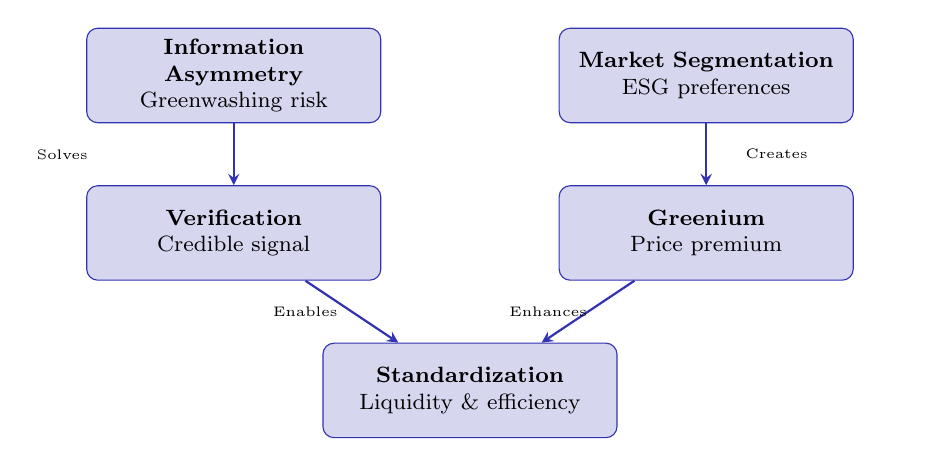
\begin{tikzpicture}[
  node distance=2cm,
  box/.style={rectangle, rounded corners, draw=mlpurple, fill=mllavender4, text width=3.5cm, align=center, minimum height=1.2cm, font=\footnotesize},
  arrow/.style={->, >=stealth, thick, color=mlpurple}
]

% Top row
\node[box] (asymmetry) at (0,4) {\textbf{Information Asymmetry}\\Greenwashing risk};
\node[box] (segmentation) at (6,4) {\textbf{Market Segmentation}\\ESG preferences};

% Middle row
\node[box] (verification) at (0,2) {\textbf{Verification}\\Credible signal};
\node[box] (greenium) at (6,2) {\textbf{Greenium}\\Price premium};

% Bottom row
\node[box] (standardization) at (3,0) {\textbf{Standardization}\\Liquidity \& efficiency};

% Arrows
\draw[arrow] (asymmetry) -- (verification);
\draw[arrow] (segmentation) -- (greenium);
\draw[arrow] (verification) -- (standardization);
\draw[arrow] (greenium) -- (standardization);

% Labels
\node[font=\tiny, text width=2cm] at (-1.5,3) {Solves};
\node[font=\tiny, text width=2cm] at (7.5,3) {Creates};
\node[font=\tiny, text width=2cm] at (1.5,1) {Enables};
\node[font=\tiny, text width=2cm] at (4.5,1) {Enhances};

\end{tikzpicture}
\end{center}
\bottomnote{[Goal 1] Complete theoretical framework showing interconnected concepts}
\end{frame}

% ============================================================
% LECTURE 2: GOAL 2 MEASUREMENT (Slides 14-24)
% ============================================================

% Slide 14: Learning Goal 2 Title
\begin{frame}[plain]
\progressbar{2}
\vfill
\centering
\begin{beamercolorbox}[sep=12pt,center]{title}
{\Huge \textbf{Learning Goal 2}}\\[1.5em]
{\Large Quantify and analyze global green finance market size, growth trajectories, and geographic distribution}\\[1em]
{\normalsize \textcolor{mllavender}{quantitative | Build - Develops empirical measurement capabilities}}
\end{beamercolorbox}
\vfill
\end{frame}

% Slide 15: Measurement Methodology
\begin{frame}[t]{Measuring the Green Finance Market}
\progressbar{2}
\begin{columns}[T]
\column{0.48\textwidth}
\textbf{Methodological Challenges}
\begin{itemize}
\item Definition: What qualifies as ``green''? (Taxonomy dependence)
\item Double counting: Issuance vs outstanding amounts
\item Currency: Conversion to common denominator (USD)
\item Coverage: Data availability varies by region and instrument
\end{itemize}

\column{0.48\textwidth}
\textbf{Standard Metrics}
\begin{itemize}
\item Total market size: Outstanding amount (stock)
\item Annual issuance: New volume each year (flow)
\item CAGR: Compound Annual Growth Rate
\item Market share: By instrument, region, sector
\end{itemize}
\end{columns}
\bottomnote{[Goal 2] Rigorous quantification requires clear methodology and consistent definitions}
\end{frame}

% Slide 16: Chart - Market Growth
\begin{frame}[t]{Global Green Finance Market Growth 2015-2024}
\progressbar{2}
\vspace{-2mm}
\begin{center}
\includegraphics[width=0.75\textwidth]{charts/week1/week1_v2_goal2_chart1_market_growth.pdf}
\end{center}
\bottomnote{[Goal 2] Market grew from \$300B (2015) to \$2.1T (2024) - This validates the growth prediction from Slide 11}
\end{frame}

% Slide 17: Growth Rate Calculation
\begin{frame}[t]{Growth Rate Analysis: CAGR Calculation}
\progressbar{2}
\begin{columns}[T]
\column{0.48\textwidth}
\textbf{CAGR Formula and Application}
\begin{itemize}
\item Formula: $CAGR = (V_{final}/V_{initial})^{1/n} - 1$
\item Period: 2015-2024 (n = 9 years)
\item Initial: \$300B (2015)
\item Final: \$2,100B (2024)
\item Calculation: $(2100/300)^{1/9} - 1 = 24.9\%$
\end{itemize}

\column{0.48\textwidth}
\textbf{Interpretation and Context}
\begin{itemize}
\item 24.9\% CAGR indicates explosive growth phase
\item Comparison: Global bond market $\sim$5\% CAGR same period
\item Green finance growing 5$\times$ faster than conventional
\item 2022 dip (\$1.45T) due to broader market volatility
\end{itemize}
\end{columns}
\bottomnote{[Goal 2] Quantitative analysis confirms theoretical prediction of rapid market expansion}
\end{frame}

% Slide 18: Chart - Regional Distribution
\begin{frame}[t]{Geographic Distribution of Green Finance}
\progressbar{2}
\begin{center}
\includegraphics[width=0.75\textwidth]{charts/week1/week1_v2_goal2_chart2_regional.pdf}
\end{center}
\bottomnote{[Goal 2] Europe 44\%, Asia-Pacific 32\%, Americas 20\% - Reflects regulatory push predicted in theory (Slide 10)}
\end{frame}

% Slide 19: Regional Analysis
\begin{frame}[t]{Regional Patterns and Drivers}
\progressbar{2}
\begin{columns}[T]
\column{0.48\textwidth}
\textbf{Europe: Market Leader}
\begin{itemize}
\item 44\% global market share (\$920B annual issuance)
\item Driver: EU Taxonomy mandatory disclosure
\item SFDR regulation creates demand from asset managers
\item Strong sovereign issuance (France, Germany, UK)
\end{itemize}

\column{0.48\textwidth}
\textbf{Asia-Pacific: Rapid Growth}
\begin{itemize}
\item 32\% market share (\$680B), fastest growth region
\item China dominates (\$450B), policy-driven expansion
\item Japan, South Korea increasing (net-zero commitments)
\item Southeast Asia emerging (ASEAN Taxonomy)
\end{itemize}
\end{columns}
\bottomnote{[Goal 2] Regional variation driven by policy frameworks and regulatory mandates}
\end{frame}

% Slide 19A: NEW - Verification Stats
\begin{frame}[t]{External Verification in Green Bond Market}
\progressbar{2}
\vspace{-10mm}
\begin{center}
\includegraphics[width=0.85\textwidth]{charts/week1/12_verification_stats/12_verification_stats.pdf}
\end{center}
\vspace{-5mm}
\bottomnote{[Goal 2] Over 80\% of green bonds have external review (OECD 2024) - validates signaling theory from Lecture 1}
\end{frame}

% Slide 20: Chart - Instrument Breakdown
\begin{frame}[t]{Market Composition by Instrument Type}
\progressbar{2}
\begin{center}
\includegraphics[width=0.75\textwidth]{charts/week1/week1_v2_goal2_chart3_instruments.pdf}
\end{center}
\bottomnote{[Goal 2] Green bonds \$1.6T (76\%), Sustainability-linked bonds \$500B (24\%) of total}
\end{frame}

% Slide 20A: NEW - Issuer Concentration
\begin{frame}[t]{Top Green Bond Issuers 2015-2024}
\progressbar{2}
\vspace{-10mm}
\begin{center}
\includegraphics[width=0.85\textwidth]{charts/week1/13_issuer_concentration/13_issuer_concentration.pdf}
\end{center}
\vspace{-5mm}
\bottomnote{[Goal 2] Repeat issuers dominate market - confirms reputation effects predicted in theory}
\end{frame}

% Slide 21: Chart - Sector Allocation
\begin{frame}[t]{Allocation Across Economic Sectors}
\progressbar{2}
\begin{center}
\includegraphics[width=0.75\textwidth]{charts/week1/week1_v2_goal2_chart4_sectors.pdf}
\end{center}
\bottomnote{[Goal 2] Energy 38\%, Buildings 24\%, Transport 18\% - aligns with decarbonization priorities}
\end{frame}

% Slide 21A: NEW - ESG Fund Flows
\begin{frame}[t]{ESG Fund Net Inflows and Assets Under Management}
\progressbar{2}
\vspace{-10mm}
\begin{center}
\includegraphics[width=0.80\textwidth]{charts/week1/15_esg_fund_flows/15_esg_fund_flows.pdf}
\end{center}
\vspace{-7mm}
\bottomnote{[Goal 2] ESG AUM grew from \$1.2T (2019) to \$3.5T (2024) - drives demand for green bonds}
\end{frame}

% Slide 22: Statistical Summary
\begin{frame}[t]{Quantitative Summary: Key Statistics}
\progressbar{2}
\begin{columns}[T]
\column{0.48\textwidth}
\textbf{Market Size Metrics (2024)}
\begin{itemize}
\item Total outstanding: \$2.1 trillion
\item Annual issuance: \$650 billion
\item Green bonds outstanding: \$1.6T (76\%)
\item Number of issuers: 1,200+ globally
\item Average deal size: \$540 million
\end{itemize}

\column{0.48\textwidth}
\textbf{Growth and Distribution}
\begin{itemize}
\item 9-year CAGR: 24.9\% (2015-2024)
\item Regional: EU 44\%, APAC 32\%, Americas 20\%
\item Sectoral: Energy 38\%, Buildings 24\%, Transport 18\%
\item Forecasted 2030: \$5.0-6.0 trillion
\end{itemize}
\end{columns}
\bottomnote{[Goal 2] Comprehensive quantitative picture validates theoretical predictions from Lecture 1}
\end{frame}

% Slide 23: Goal 2 Summary
\begin{frame}[t]{Learning Goal 2: Summary}
\progressbar{2}
\begin{center}
{\Large \textbf{Learning Goal 2: Summary}}\\[0.5em]
{\normalsize \textit{Quantify and analyze market size, growth, and distribution}}
\end{center}

\vspace{0.5em}

\begin{columns}[T]
\column{0.48\textwidth}
\textbf{What We Achieved}
\begin{itemize}
\item \textcolor{mlgreen}{$\checkmark$} Quantified market at \$2.1T with 24.9\% CAGR (2015-2024)
\item \textcolor{mlgreen}{$\checkmark$} Analyzed regional distribution: Europe leads (44\%), Asia growing fastest
\item \textcolor{mlgreen}{$\checkmark$} Measured instrument composition: Green bonds dominant (76\%)
\item \textcolor{mlgreen}{$\checkmark$} Validated theoretical predictions with empirical data
\end{itemize}

\column{0.48\textwidth}
\textbf{Can You Now...}
\begin{itemize}
\item Calculate growth rates (CAGR) for market segments?
\item Compare regional adoption and explain differences?
\item Analyze sector allocation and investment priorities?
\item Use empirical data to test theoretical hypotheses?
\end{itemize}
\end{columns}

\bottomnote{[Goal 2] Achieved - Quantitative measurement complete. Next: Mathematical valuation models}
\end{frame}

% Slide 24: NEW - Concept Map Lecture 2
\begin{frame}[t]{Concept Map: Theory + Evidence Integration}
\progressbar{2}
\begin{center}
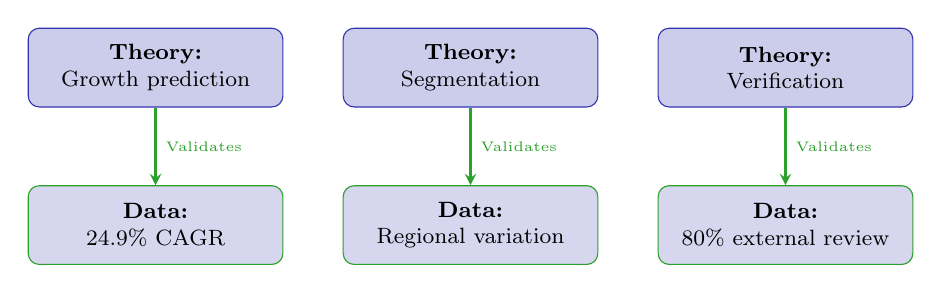
\begin{tikzpicture}[
  node distance=2.5cm,
  theory/.style={rectangle, rounded corners, draw=mlpurple, fill=mllavender3, text width=3cm, align=center, minimum height=1cm, font=\footnotesize},
  evidence/.style={rectangle, rounded corners, draw=mlgreen, fill=mllavender4, text width=3cm, align=center, minimum height=1cm, font=\footnotesize},
  arrow/.style={->, >=stealth, thick}
]

% Top row - Theory
\node[theory] (t1) at (0,3) {\textbf{Theory:}\\Growth prediction};
\node[theory] (t2) at (4,3) {\textbf{Theory:}\\Segmentation};
\node[theory] (t3) at (8,3) {\textbf{Theory:}\\Verification};

% Bottom row - Evidence
\node[evidence] (e1) at (0,1) {\textbf{Data:}\\24.9\% CAGR};
\node[evidence] (e2) at (4,1) {\textbf{Data:}\\Regional variation};
\node[evidence] (e3) at (8,1) {\textbf{Data:}\\80\% external review};

% Arrows
\draw[arrow, color=mlgreen] (t1) -- (e1) node[midway, right, font=\tiny] {Validates};
\draw[arrow, color=mlgreen] (t2) -- (e2) node[midway, right, font=\tiny] {Validates};
\draw[arrow, color=mlgreen] (t3) -- (e3) node[midway, right, font=\tiny] {Validates};

\end{tikzpicture}
\end{center}
\bottomnote{[Goal 2] Theory validated by data - Strong empirical foundation for valuation models}
\end{frame}

% ============================================================
% LECTURE 3: GOAL 3 VALUATION PART 1 (Slides 25-32)
% ============================================================

% Slide 25: Learning Goal 3 Title
\begin{frame}[plain]
\progressbar{3}
\vfill
\centering
\begin{beamercolorbox}[sep=12pt,center]{title}
{\Huge \textbf{Learning Goal 3}}\\[1.5em]
{\Large Derive and apply bond pricing models incorporating greenium and environmental premium adjustments}\\[1em]
{\normalsize \textcolor{mllavender}{mathematical | Apply - Demonstrates mathematical valuation methods}}
\end{beamercolorbox}
\vfill
\end{frame}

% Slide 26: Classical Pricing Derivation
\begin{frame}[t]{Classical Bond Pricing: Derivation from First Principles}
\progressbar{3}
\begin{columns}[T]
\column{0.48\textwidth}
\textbf{Starting Point}

$$P_0 = \sum_{t=1}^{T} \frac{C}{(1+r)^t} + \frac{F}{(1+r)^T}$$

\textbf{Assumptions:}
\begin{itemize}
\item Constant discount rate $r$ (risk-free + credit spread)
\item Fixed annual coupon $C$
\item Face value $F$ repaid at maturity $T$
\item No embedded options or default
\end{itemize}

\column{0.48\textwidth}
\textbf{Algebraic Simplification}

\begin{enumerate}
\item Separate coupon annuity from principal:
\begin{equation*}
P_0 = C \sum_{t=1}^{T} (1+r)^{-t} + F(1+r)^{-T}
\end{equation*}

\item Apply geometric series formula to annuity:
\begin{equation*}
= C \cdot \frac{1 - (1+r)^{-T}}{r} + F(1+r)^{-T}
\end{equation*}

\item Standard decomposition for analysis:
\begin{equation*}
= PV(\text{Coupons}) + PV(\text{Principal})
\end{equation*}
\end{enumerate}
\end{columns}
\bottomnote{[Goal 3] Classical formula forms mathematical foundation for all bond valuation}
\end{frame}

% Slide 27: Greenium Incorporation
\begin{frame}[t]{Green Bond Pricing: Incorporating Greenium}
\progressbar{3}
\begin{columns}[T]
\column{0.48\textwidth}
\textbf{Theoretical Extension}

$$P_G = \sum_{t=1}^{T} \frac{C}{(1+r-g)^t} + \frac{F}{(1+r-g)^T}$$

\textbf{Key Elements:}
\begin{itemize}
\item Greenium $g > 0$ (0-5 bps typically)
\item Same cash flows as conventional bond
\item Environmental premium priced via lower required return
\item Adjust discount rate by greenium $g$
\end{itemize}

\column{0.48\textwidth}
\textbf{Price Differential Analysis}

\begin{enumerate}
\item Green bond trades at premium:
\begin{equation*}
P_G > P_0 \text{ if } g > 0
\end{equation*}

\item Convert decimal to basis points:
\begin{equation*}
\text{Greenium (bps)} = g \times 10000
\end{equation*}

\item Price difference approximation using duration $D$:
\begin{equation*}
P_G - P_0 \approx C \cdot g \cdot D
\end{equation*}
\end{enumerate}
\end{columns}
\bottomnote{[Goal 3] Mathematical model quantifies greenium's impact on bond valuation}
\end{frame}

% Slide 28: Worked Example
\begin{frame}[t]{Numerical Example: Green vs Conventional Pricing}
\progressbar{3}
\begin{columns}[T]
\column{0.48\textwidth}
\textbf{Bond Specifications}
\begin{itemize}
\item Face value: $F = 1000$ (EUR)
\item Coupon rate: 3\% annual (C = 30 EUR)
\item Maturity: T = 10 years
\item Risk-free rate: 2\%
\item Credit spread: 0.5\%
\item Greenium: g = 0.03\% (3 bps)
\end{itemize}

\column{0.48\textwidth}
\textbf{Valuation Calculations}
\begin{itemize}
\item Conventional: $r = 2.5\%$
\item Price: $P_0 = 1043.76$ EUR
\item Green: $r_G = 2.47\%$ (2.5\% - 0.03\%)
\item Price: $P_G = 1046.89$ EUR
\item Difference: $3.13$ EUR (0.3\% premium)
\end{itemize}

\vspace{1em}
\begin{beamercolorbox}[sep=8pt,center]{block body}
\textbf{Try it yourself:} Calculate price for greenium = 5 bps\\
\textit{Answer: $P_G = 1048.98$ EUR (5.22 EUR premium)}
\end{beamercolorbox}
\end{columns}
\bottomnote{[Goal 3] 3 bps greenium translates to €3.13 price premium on €1000 bond}
\end{frame}

% Slide 29: Chart - Yield Comparison
\begin{frame}[t]{Yield Curves: Green vs Conventional Bonds}
\progressbar{3}
\vspace{-2mm}
\begin{center}
\includegraphics[width=0.75\textwidth]{charts/week1/week1_v2_goal3_chart1_yields.pdf}
\end{center}
\bottomnote{[Goal 3] Greenium of 3-4 bps confirms segmentation theory (Slide 8) - Empirical validation of theory}
\end{frame}

% Slide 30: Duration and Sensitivity
\begin{frame}[t]{Duration Analysis and Price Sensitivity}
\progressbar{3}
\begin{columns}[T]
\column{0.48\textwidth}
\textbf{Modified Duration}
\begin{itemize}
\item Duration $D = \frac{1}{P} \frac{\partial P}{\partial r}$
\item Measures price sensitivity to yield changes
\item Higher duration $\rightarrow$ greater greenium impact
\item 10-year bond: $D \approx 8.5$ years
\end{itemize}

\column{0.48\textwidth}
\textbf{Greenium Sensitivity}
\begin{itemize}
\item Price change: $\Delta P \approx -P \cdot D \cdot \Delta r$
\item 1 bp greenium on 10-yr bond: 0.085\% price impact
\item Longer maturity amplifies greenium effect
\item Investor arbitrage limited by segmentation
\end{itemize}
\end{columns}
\bottomnote{[Goal 3] Mathematical relationship validates pricing framework - Duration increases greenium impact}
\end{frame}

% Slide 31: Chart - Duration Model
\begin{frame}[t]{Pricing Model: Green Premium vs Duration}
\progressbar{3}
\vspace{-2mm}
\begin{center}
\includegraphics[width=0.75\textwidth]{charts/week1/week1_v2_goal3_chart2_duration.pdf}
\end{center}
\bottomnote{[Goal 3] Longer duration bonds show larger absolute price premium for given greenium}
\end{frame}

% Slide 32: Risk-Return Framework
\begin{frame}[t]{Risk-Return Analysis for Green Bonds}
\progressbar{3}
\begin{columns}[T]
\column{0.48\textwidth}
\textbf{Return Components}
\begin{itemize}
\item Base return: Risk-free rate + credit spread
\item Greenium effect: Lower required return (-3 to -5 bps)
\item Liquidity premium: May offset greenium (varies)
\item Total return: Comparable to conventional bonds
\end{itemize}

\column{0.48\textwidth}
\textbf{Risk Profile}
\begin{itemize}
\item Credit risk: Identical to conventional bonds (same issuer)
\item Interest rate risk: Measured by duration (same as conventional)
\item Greenwashing risk: Specific to green bonds (mitigated by verification)
\item Regulatory risk: EU Taxonomy changes, standards evolution
\end{itemize}
\end{columns}
\bottomnote{[Goal 3] Green bonds offer similar risk-return profile with additional ESG benefit}
\end{frame}

% ============================================================
% LECTURE 4: GOAL 3 PART 2 + APPLICATIONS (Slides 33-42)
% ============================================================

% Slide 33: Chart - Risk-Return Scatter
\begin{frame}[t]{Risk-Return Profile: Green vs Conventional}
\progressbar{4}
\vspace{-2mm}
\begin{center}
\includegraphics[width=0.75\textwidth]{charts/week1/week1_v2_goal3_chart3_risk_return.pdf}
\end{center}
\bottomnote{[Goal 3] Empirical evidence: Competitive risk-adjusted returns with lower volatility}
\end{frame}

% Slide 34: Chart - Greenium Over Time
\begin{frame}[t]{Greenium Evolution 2019-2024}
\progressbar{4}
\vspace{-2mm}
\begin{center}
\includegraphics[width=0.75\textwidth]{charts/week1/week1_v2_goal3_chart4_greenium_time.pdf}
\end{center}
\bottomnote{[Goal 3] Greenium declining from 7 bps (2019) to 2 bps (2024) as supply meets demand}
\end{frame}

% Slide 35: Week Summary (All 3 Goals Integrated)
\begin{frame}[t]{Week 1 Complete: Theory $\rightarrow$ Measurement $\rightarrow$ Valuation}
\progressbar{4}
\begin{center}
{\Large \textbf{Week 1 Integration: Complete Green Finance Foundation}}
\end{center}

\vspace{0.5em}

\begin{columns}[T]
\column{0.48\textwidth}
\textbf{Three-Goal Narrative Complete}
\begin{itemize}
\item \textcolor{mlgreen}{$\checkmark$} Goal 1 (Theory): WHY green finance exists - information asymmetry, segmentation
\item \textcolor{mlgreen}{$\checkmark$} Goal 2 (Measurement): HOW MUCH - \$2.1T market, 25\% CAGR, geographic distribution
\item \textcolor{mlgreen}{$\checkmark$} Goal 3 (Valuation): HOW TO PRICE - pricing models, greenium quantification
\item \textcolor{mlgreen}{$\checkmark$} Story arc: Theoretical foundation $\rightarrow$ Empirical evidence $\rightarrow$ Mathematical application
\end{itemize}

\column{0.48\textwidth}
\textbf{Week 1 Mastery: Can You...}
\begin{itemize}
\item Explain greenium using microstructure theory?
\item Calculate market growth rates and project future size?
\item Derive bond pricing models and apply to green bonds?
\item Integrate theory, data, and mathematics in analysis?
\end{itemize}
\end{columns}

\vspace{0.5em}

\bottomnote{Week 1 foundations complete - Integrated theoretical, empirical, and mathematical frameworks}
\end{frame}

% Slide 36: NEW - Credit Ratings
\begin{frame}[t]{Credit Rating Distribution: Green vs Conventional}
\progressbar{4}
\vspace{-10mm}
\begin{center}
\includegraphics[width=0.85\textwidth]{charts/week1/14_credit_ratings/14_credit_ratings.pdf}
\end{center}
\vspace{-5mm}
\bottomnote{[Goal 3] Green bonds show higher credit quality (predominantly investment grade) - Lower credit risk}
\end{frame}

% Slide 37: NEW - Standardization
\begin{frame}[t]{Standardization in Green Bond Market}
\progressbar{4}
\vspace{-10mm}
\begin{center}
\includegraphics[width=0.85\textwidth]{charts/week1/16_standardization/16_standardization.pdf}
\end{center}
\vspace{-5mm}
\bottomnote{[Goal 1] 96\% of market follows established standards - Validates standardization theory from Slide 10}
\end{frame}

% Slide 38: NEW - Verification Revisited
\begin{frame}[t]{External Verification in Green Bond Market (Revisited)}
\progressbar{4}
\vspace{-10mm}
\begin{center}
\includegraphics[width=0.85\textwidth]{charts/week1/12_verification_stats/12_verification_stats.pdf}
\end{center}
\vspace{-5mm}
\bottomnote{[Goal 1] Verification as credible signal - Theory from Slide 7 empirically confirmed}
\end{frame}

% Slide 39: NEW - Complete Concept Map
\begin{frame}[t]{Complete Integration: All 4 Lectures Connected}
\progressbar{4}
\begin{center}
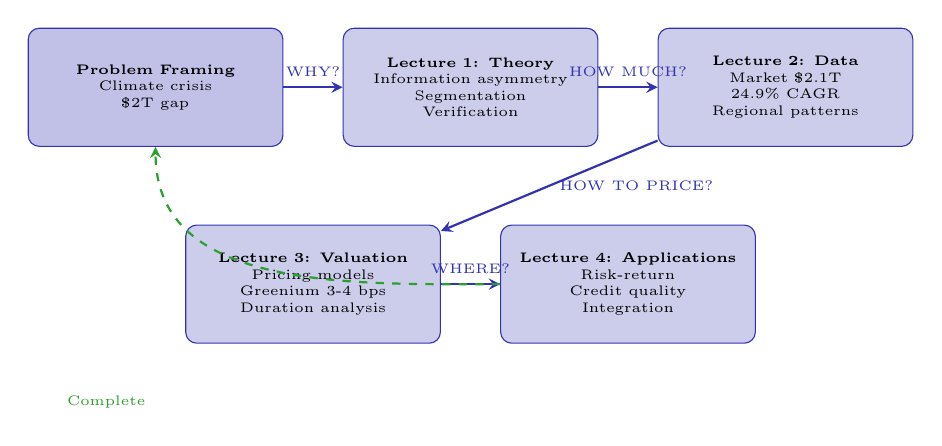
\begin{tikzpicture}[
  node distance=1.5cm,
  lecture/.style={rectangle, rounded corners, draw=mlpurple, fill=mllavender3, text width=3cm, align=center, minimum height=1.5cm, font=\tiny},
  arrow/.style={->, >=stealth, thick, color=mlpurple}
]

% Four lectures in a flow
\node[lecture, fill=mllavender2] (l0) at (0,4) {\textbf{Problem Framing}\\Climate crisis\\\$2T gap};
\node[lecture] (l1) at (4,4) {\textbf{Lecture 1: Theory}\\Information asymmetry\\Segmentation\\Verification};
\node[lecture] (l2) at (8,4) {\textbf{Lecture 2: Data}\\Market \$2.1T\\24.9\% CAGR\\Regional patterns};
\node[lecture] (l3) at (2,1.5) {\textbf{Lecture 3: Valuation}\\Pricing models\\Greenium 3-4 bps\\Duration analysis};
\node[lecture] (l4) at (6,1.5) {\textbf{Lecture 4: Applications}\\Risk-return\\Credit quality\\Integration};

% Flow arrows
\draw[arrow] (l0) -- (l1) node[midway, above, font=\tiny] {WHY?};
\draw[arrow] (l1) -- (l2) node[midway, above, font=\tiny] {HOW MUCH?};
\draw[arrow] (l2) -- (l3) node[midway, right, font=\tiny] {HOW TO PRICE?};
\draw[arrow] (l3) -- (l4) node[midway, above, font=\tiny] {WHERE?};

% Feedback loop
\draw[arrow, dashed, color=mlgreen] (l4) to[out=180,in=270] (l0) node[midway, left, font=\tiny] {Complete};

\end{tikzpicture}
\end{center}
\bottomnote{[All Goals] Complete journey from problem to application - Theory-Evidence-Mathematics integrated}
\end{frame}

% Slide 40: NEW - Portfolio Exercise
\begin{frame}[t]{Portfolio Exercise: Where Would You Invest?}
\progressbar{4}
\begin{center}
{\large \textbf{Interactive Risk-Return Positioning}}
\end{center}

\vspace{0.5em}

\begin{columns}[T]
\column{0.48\textwidth}
\textbf{Investment Options}
\begin{enumerate}
\item German green sovereign (10-yr, AAA, 3 bps greenium)
\item France green corporate (5-yr, A, 4 bps greenium)
\item China green development (7-yr, BBB+, 5 bps greenium)
\item US sustainability-linked (10-yr, AA, 2 bps greenium)
\end{enumerate}

\vspace{0.5em}

\textbf{Your Constraints}
\begin{itemize}
\item Target duration: 7-8 years
\item Risk appetite: Investment grade only
\item ESG preference: High greenium preferred
\end{itemize}

\column{0.48\textwidth}
\textbf{Decision Framework}
\begin{itemize}
\item Apply Goal 3 pricing models
\item Consider Goal 1 theoretical predictions
\item Use Goal 2 market data for context
\item Evaluate credit risk vs greenium trade-off
\end{itemize}

\vspace{1em}

\begin{beamercolorbox}[sep=8pt,center]{block body}
\textbf{Recommended:} China green development\\
\textit{Rationale: Optimal duration (7 yrs), investment grade, highest greenium (5 bps), growing market}
\end{beamercolorbox}
\end{columns}

\bottomnote{[Application] Integrate all three goals to make informed investment decisions}
\end{frame}

% Slide 41: NEW - Case Study
\begin{frame}[t]{Real-World Application: France's Green Sovereign Bond}
\progressbar{4}
\begin{columns}[T]
\column{0.48\textwidth}
\textbf{Transaction Details (2017-2024)}
\begin{itemize}
\item First sovereign green bond: January 2017
\item Total issuance: \$85 billion (2017-2024)
\item Maturity range: 10-25 years
\item Average greenium: 3-5 bps at issuance
\item Use of proceeds: Energy transition, sustainable transport
\end{itemize}

\vspace{0.5em}

\textbf{Market Impact}
\begin{itemize}
\item Oversubscribed 7$\times$ on average
\item Attracted new ESG-dedicated investors
\item Set benchmark for sovereign green issuance
\end{itemize}

\column{0.48\textwidth}
\textbf{How Theory Explains Success}
\begin{itemize}
\item \textbf{Goal 1:} AAA rating + verification = credible signal reducing information asymmetry
\item \textbf{Goal 2:} Large issue size (\$7B+) = liquidity premium + standardization benefits
\item \textbf{Goal 3:} Greenium 3-5 bps = competitive pricing attracting ESG-segmented investors
\end{itemize}

\vspace{0.5em}

\textbf{Outcomes}
\begin{itemize}
\item Successful funding: \$85B mobilized for climate
\item Market leadership: France top sovereign issuer
\item Demonstrated scalability of green finance
\end{itemize}
\end{columns}

\bottomnote{[Application] France case integrates all theoretical, empirical, and valuation concepts from Week 1}
\end{frame}

% Slide 42: NEW - Next Week Preview
\begin{frame}[t]{Looking Ahead: Week 2 Preview}
\progressbar{4}
\begin{columns}[T]
\column{0.48\textwidth}
\textbf{What We Accomplished in Week 1}
\begin{itemize}
\item Built theoretical foundation (microstructure theory)
\item Quantified global market (\$2.1T, 25\% CAGR)
\item Derived mathematical pricing models
\item Applied framework to real investments
\end{itemize}

\vspace{0.5em}

\textbf{Open Questions for Week 2}
\begin{itemize}
\item How are green bonds actually structured?
\item What is the issuance process step-by-step?
\item How do taxonomies define ``green''?
\item What role do third-party verifiers play?
\end{itemize}

\column{0.48\textwidth}
\textbf{Week 2 Focus: Green Bond Structures}
\begin{itemize}
\item Issuance lifecycle and documentation
\item Green Bond Principles (ICMA framework)
\item Taxonomy alignment (EU, China, ASEAN)
\item Verification and certification processes
\item Impact reporting requirements
\end{itemize}

\vspace{0.5em}

\textbf{Building on Week 1}
\begin{itemize}
\item Week 1: WHY and HOW MUCH (macro view)
\item Week 2: WHAT and HOW (micro implementation)
\item Integration: Theory $\rightarrow$ Practice
\end{itemize}
\end{columns}

\bottomnote{Week 2 deepens understanding by examining operational details of green bond issuance and standards}
\end{frame}

\end{document}
